%latex model.tex
%bibtex model
%latex model.tex
%latex model.tex
%dvipdfm model.dvi

%se poate lucra si online (de ex www.overleaf.com)


\documentclass[runningheads,a4paper,11pt]{report}

\usepackage{algorithmic}
\usepackage{algorithm} 
\usepackage{array}
\usepackage{amsmath}
\usepackage{amsfonts}
\usepackage{amssymb}
\usepackage{amsthm}
\usepackage{caption}
\usepackage{comment} 
\usepackage{epsfig} 
\usepackage{fancyhdr}
\usepackage[T1]{fontenc}
\usepackage{geometry} 
\usepackage{graphicx}
\usepackage[colorlinks]{hyperref} 
\usepackage[latin1]{inputenc}
\usepackage{multicol}
\usepackage{multirow} 
\usepackage{rotating}
\usepackage{setspace}
\usepackage{subfigure}
\usepackage{url}
\usepackage{verbatim}
\usepackage{xcolor}

\geometry{a4paper,top=3cm,left=2cm,right=2cm,bottom=3cm}

\pagestyle{fancy}
\fancyhf{}
\fancyhead[LE,RO]{Project's name}
\fancyhead[RE,LO]{Team's name}
\fancyfoot[RE,LO]{MIRPR 2019-2020}
\fancyfoot[LE,RO]{\thepage}

\renewcommand{\headrulewidth}{2pt}
\renewcommand{\footrulewidth}{1pt}
\renewcommand{\headrule}{\hbox to\headwidth{%
  \color{lime}\leaders\hrule height \headrulewidth\hfill}}
\renewcommand{\footrule}{\hbox to\headwidth{%
  \color{lime}\leaders\hrule height \footrulewidth\hfill}}

\hypersetup{
pdftitle={artTitle},
pdfauthor={name},
pdfkeywords={pdf, latex, tex, ps2pdf, dvipdfm, pdflatex},
bookmarksnumbered,
pdfstartview={FitH},
urlcolor=cyan,
colorlinks=true,
linkcolor=red,
citecolor=green,
}
% \pagestyle{plain}

\setcounter{secnumdepth}{3}
\setcounter{tocdepth}{3}

\linespread{1}

% \pagestyle{myheadings}

\makeindex


\begin{document}

\begin{titlepage}
\sloppy
\begin{center}
BABE\c S BOLYAI UNIVERSITY, CLUJ NAPOCA, ROM\^ ANIA

FACULTY OF MATHEMATICS AND COMPUTER SCIENCE

\vspace{6cm}

\Huge \textbf{TITLE}

\vspace{1cm}

\normalsize -- MIRPR report --

\end{center}


\vspace{5cm}

\begin{flushright}
\Large{\textbf{Team members}}\\
Name, specialisation, group
\end{flushright}

\vspace{4cm}

\begin{center}
2019
\end{center}

\end{titlepage}

\pagenumbering{gobble}

\begin{abstract}
	Text of abstract. Short info about: project relevance/importance, inteligent methods used for solving, data involved in the numerical experiments; conclude by the the results obtained.
\end{abstract}


\tableofcontents

\newpage

\listoftables
\listoffigures
\listofalgorithms

\newpage

\setstretch{1.5}



\newpage

\pagenumbering{arabic}


 


\chapter{Introduction}
\label{chapter:introduction}

\section{What? Why? How?}
\label{section:what}

Motivate and abstractly describe the problem you are addressing and how you are addressing it. 
\begin{itemize}
	\item What is the (scientific) problem? 
	\item Why is it important? 
	\item What is your basic approach? 
\end{itemize}

A short discussion of how it fits into related work in the area is also desirable. Summarize the basic results and conclusions that you will present. 


\section{Paper structure and original contribution(s)}
\label{section:structure}

The research presented in this paper advances the theory, design, and implementation of several particular models. 

The main contribution of this report is to present an intelligent algorithm for solving the problem of $\ldots$.

The second contribution of this report consists of building an intuitive, easy-to-use and user
friendly software application. Our aim is to build an algorithm that will help $\ldots$.

The third contribution of this thesis consists of $\ldots$.


The present work contains $xyz$ bibliographical references and is structured in five chapters as follows.

The first chapter/section is a short introduction in $\ldots$.

The second chapter/section describes $\ldots$.

The chapter/section \ref{chapter:proposedApproach} details $\ldots$.



\chapter{Scientific Problem}
\label{section:scientificProblem}


\section{Problem definition}
\label{section:problemDefinition}

Give a description of the problem.
Explain why it must be solved by an intelligent algorithm. 
Details the advantages and/or disadvantages of solving the problem by a (some) given method(s).

Precisely define the problem you are addressing (i.e. formally specify the inputs and outputs). Elaborate on why this is an interesting and important problem.


Item example: 

\begin{itemize}
	\item content of item1
 	\item content of item2
 	\item content of item3
\end{itemize}



Figure example 

$\ldots$ (see Figure \ref{swarmsize})

\begin{figure}[htbp]
	\centerline{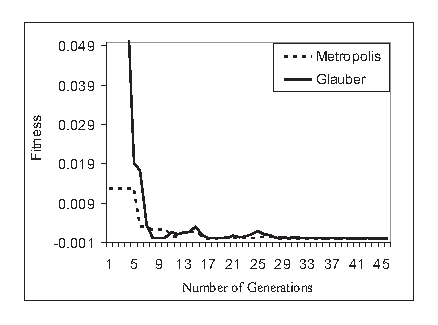
\includegraphics{Fig/FitEvol.eps}}  
	\caption{The evolution of the swarm size during the GA generations. This results were obtained for the $f_2$ test function with 5 dimensions.}
	\label{swarmsize}
\end{figure}


Table example: (see Table \ref{tab3PSO})


\begin{table}[htbp]
	\caption{The parameters of the PSO algorithm (the micro level algorithm) used to compute the fitness of a GA chromosome.}
	\label{tab3PSO}
		\begin{center}
			\begin{tabular}{p{220pt}c}

				\textbf{Parameter}& \textbf{Value} \\
				\hline\hline
 				Number of generations& 50 \\
 				Number of function evaluations/generation& 10 \\
 				Number of dimensions of the function to be optimized& 5 \\
 				Learning factor $c_{1}$& 2 \\
 				Learning factor $c_{2}$ & 1.8\\
 				Inertia weight& 0.5 + $\frac{rand()}{2}$\\
		
			\end{tabular}
		\end{center}
\end{table}

Algorithm example 

$\ldots$ (see Algorithm \ref{NGalg}).


\algsetup{indent=1em, linenosize=\footnotesize}

\begin{algorithm}
	\caption{SGA - Spin based Genetic AQlgorithm}
	\label{NGalg}
		\begin{algorithmic}


			\STATE \textbf{BEGIN}
  		\STATE @ Randomly create the initial GA population.
  		\STATE @ Compute the fitness of each individual.
  		\FOR{i=1 TO NoOfGenerations}
  			\FOR{j=1 TO PopulationSize}
  				\STATE p $\leftarrow$ RandomlySelectParticleFromGrid();
  				\STATE n $\leftarrow$ RandomlySelectParticleFromNeighbors(p);
  				\STATE @ Crossover(p, n, off);
  				\STATE @ Compute energy $\Delta H$
  				\IF {$\Delta H$ satisfy the Ising condition}
  					\STATE @ Replace(p,off);
  				\ENDIF
  			\ENDFOR
  		\ENDFOR
  		\STATE \textbf{END}
\end{algorithmic}
\end{algorithm}


\chapter{State of art/Related work}
\label{chapter:stateOfArt}


The theory of the methods utilised until now in order to solve the given problem.

Answer the following questions for each piece of related work that addresses the same or a similar problem. 
\begin{itemize}
	\item What is their problem and method? 
	\item How is your problem and method different? 
	\item Why is your problem and method better?
\end{itemize}

In order to cite a given work you can use a bib file (see the example) and the $\ $ \textit{cite} command:
\cite{kennedy1}, \cite{Koh06}, \cite{Berlekamp82}, \cite{Storn95}, \cite{firefox}.



\chapter{Proposed approach}
\label{chapter:proposedApproach}

Describe your approach!

Describe in reasonable detail the algorithm you are using to address this problem. A psuedocode description of the algorithm you are using is frequently useful. Trace through a concrete example, showing how your algorithm processes this example. The example should be complex enough to illustrate all of the important aspects of the problem but simple enough to be easily understood. If possible, an intuitively meaningful example is better than one with meaningless symbols.


\chapter{Application (numerical validation)}
\label{chapter:application}


Explain the experimental methodology and the numerical results obtained with your approach and the state of art approache(s).

Try to perform a comparison of several approaches.

Statistical validation of the results.


\section{Methodology}
\label{section:methodology}

\begin{itemize}
	\item What are criteria you are using to evaluate your method? 
	\item What specific hypotheses does your experiment test? Describe the experimental methodology that you used. 
	\item What are the dependent and independent variables? 
	\item What is the training/test data that was used, and why is it realistic or interesting? Exactly what performance data did you collect and how are you presenting and analyzing it? Comparisons to competing methods that address the same problem are particularly useful.
\end{itemize}

\section{Data}
\label{section:data}

Describe the used data.

\section{Results}
\label{section:results}

Present the quantitative results of your experiments. Graphical data presentation such as graphs and histograms are frequently better than tables. What are the basic differences revealed in the data. Are they statistically significant?

\section{Discussion}
\label{section:discussion}

\begin{itemize}
	\item Is your hypothesis supported? 
	\item What conclusions do the results support about the strengths and weaknesses of your method compared to other methods? 
	\item How can the results be explained in terms of the underlying properties of the algorithm and/or the data. 
\end{itemize}



\chapter{Conclusion and future work}
\label{chapter:concl}

Try to emphasise the strengths and the weaknesses of your approach.
What are the major shortcomings of your current method? For each shortcoming, propose additions or enhancements that would help overcome it. 

Briefly summarize the important results and conclusions presented in the paper. 

\begin{itemize}
	\item What are the most important points illustrated by your work? 
	\item How will your results improve future research and applications in the area? 
\end{itemize}


\bibliographystyle{plain}
\bibliography{BibAll}

\end{document}
 
